% !TEX root = ../main.tex
% File: chapters_part1/chap5_2.tex
% Nội dung cho Chương 5, Phần 2

\section{Kỹ thuật Tinh chỉnh Hiệu quả Tham số (PEFT)}
\label{sec:peft}

Như đã phân tích ở mục trước, Tinh chỉnh Toàn bộ (Full Fine-tuning) trở nên cực kỳ tốn kém và không thực tế khi làm việc với các Mô hình Ngôn ngữ Lớn (LLMs) có hàng tỷ tham số. Việc lưu trữ và triển khai hàng chục bản sao đầy đủ của một mô hình 175 tỷ tham số cho các tác vụ khác nhau là một cơn ác mộng về mặt tài chính và kỹ thuật.

\textbf{Kỹ thuật Tinh chỉnh Hiệu quả Tham số (Parameter-Efficient Fine-Tuning - PEFT)} ra đời như một giải pháp cho vấn đề này.

\begin{tcolorbox}[
    title=Triết lý của PEFT,
    colback=green!5!white, colframe=green!60!black, fonttitle=\bfseries
]
Thay vì cập nhật \textbf{tất cả} các trọng số của mô hình lớn, chúng ta hãy \textbf{đóng băng (freeze)} toàn bộ mô hình gốc và chỉ huấn luyện một số lượng rất nhỏ các tham số \textbf{bổ sung (additional)} hoặc một \textbf{tập con} các tham số hiện có.
\end{tcolorbox}

Mục tiêu là đạt được hiệu năng gần bằng hoặc thậm chí tốt hơn Full Fine-tuning, trong khi chỉ cần huấn luyện và lưu trữ một phần rất nhỏ (thường < 1\%) của tổng số tham số. Điều này làm cho việc thích ứng LLM trở nên khả thi và hiệu quả hơn rất nhiều.

Có nhiều họ phương pháp PEFT khác nhau, chúng ta sẽ khám phá những phương pháp tiêu biểu và có ảnh hưởng nhất.

\subsection{LoRA: Thích ứng Thứ hạng Thấp (Low-Rank Adaptation)}
\label{ssec:lora}
LoRA (Hu et al., 2021) \cite{hu2021lora} là một trong những kỹ thuật PEFT phổ biến và thành công nhất hiện nay. Nó dựa trên một quan sát sâu sắc về cách các mạng nơ-ron học.

\subsubsection{Trực giác và Nền tảng Lý thuyết}
\begin{itemize}
    \item \textbf{Quan sát:} Các nhà nghiên cứu phát hiện ra rằng mặc dù các mô hình ngôn ngữ lớn có số chiều rất cao, nhưng sự thay đổi của các trọng số trong quá trình tinh chỉnh (tức là ma trận $\Delta W = W_{\text{fine-tuned}} - W_{\text{pre-trained}}$) thường có một "thứ hạng nội tại" (intrinsic rank) rất thấp.
    \item \textbf{Ý nghĩa:} Điều này có nghĩa là ma trận thay đổi trọng số $\Delta W$ (kích thước $d \times d$) có thể được xấp xỉ rất tốt bằng tích của hai ma trận nhỏ hơn nhiều, $A$ (kích thước $d \times r$) và $B$ (kích thước $r \times d$), trong đó $r$ (thứ hạng) là một số rất nhỏ so với $d$ (ví dụ: $r=8, d=4096$).
    \item \textbf{Kết luận:} Thay vì học ma trận $\Delta W$ khổng lồ với $d^2$ tham số, chúng ta có thể chỉ cần học hai ma trận nhỏ $A$ và $B$ với tổng số tham số chỉ là $2 \times d \times r$. Đây là một sự tiết kiệm rất lớn.
\end{itemize}

\subsubsection{Cơ chế hoạt động của LoRA}
LoRA áp dụng ý tưởng này vào các lớp cần nhiều tham số nhất trong Transformer, thường là các ma trận trọng số của các lớp tuyến tính trong cơ chế Self-Attention ($W_Q, W_K, W_V, W_O$).
\begin{enumerate}
    \item \textbf{Đóng băng mô hình gốc:} Toàn bộ trọng số của mô hình đã huấn luyện trước, $W_0$, được giữ nguyên và không cập nhật trong quá trình huấn luyện.
    \item \textbf{Thêm các ma trận phân rã:} Với mỗi ma trận trọng số $W_0$ mà chúng ta muốn thích ứng (ví dụ, $W_Q$), LoRA thêm vào hai ma trận "adapter" nhỏ là $A$ (khởi tạo ngẫu nhiên) và $B$ (khởi tạo bằng 0).
    \item \textbf{Sửa đổi quá trình truyền thẳng (Forward Pass):} Đầu ra của lớp được sửa đổi như sau:
        $$ h = W_0 x + \Delta W x = W_0 x + BAx $$
        Vector đầu vào $x$ sẽ đi qua hai nhánh song song:
        \begin{itemize}
            \item Nhánh chính đi qua ma trận $W_0$ đã đóng băng.
            \item Nhánh LoRA đi qua ma trận $A$ trước (giảm chiều từ $d$ xuống $r$), sau đó qua ma trận $B$ (tăng chiều từ $r$ trở lại $d$).
        \end{itemize}
        Kết quả của hai nhánh này sau đó được cộng lại với nhau.
    \item \textbf{Huấn luyện:} Chỉ có các ma trận $A$ và $B$ được huấn luyện. Tất cả các tham số khác đều bị đóng băng.
\end{enumerate}

\begin{center}
    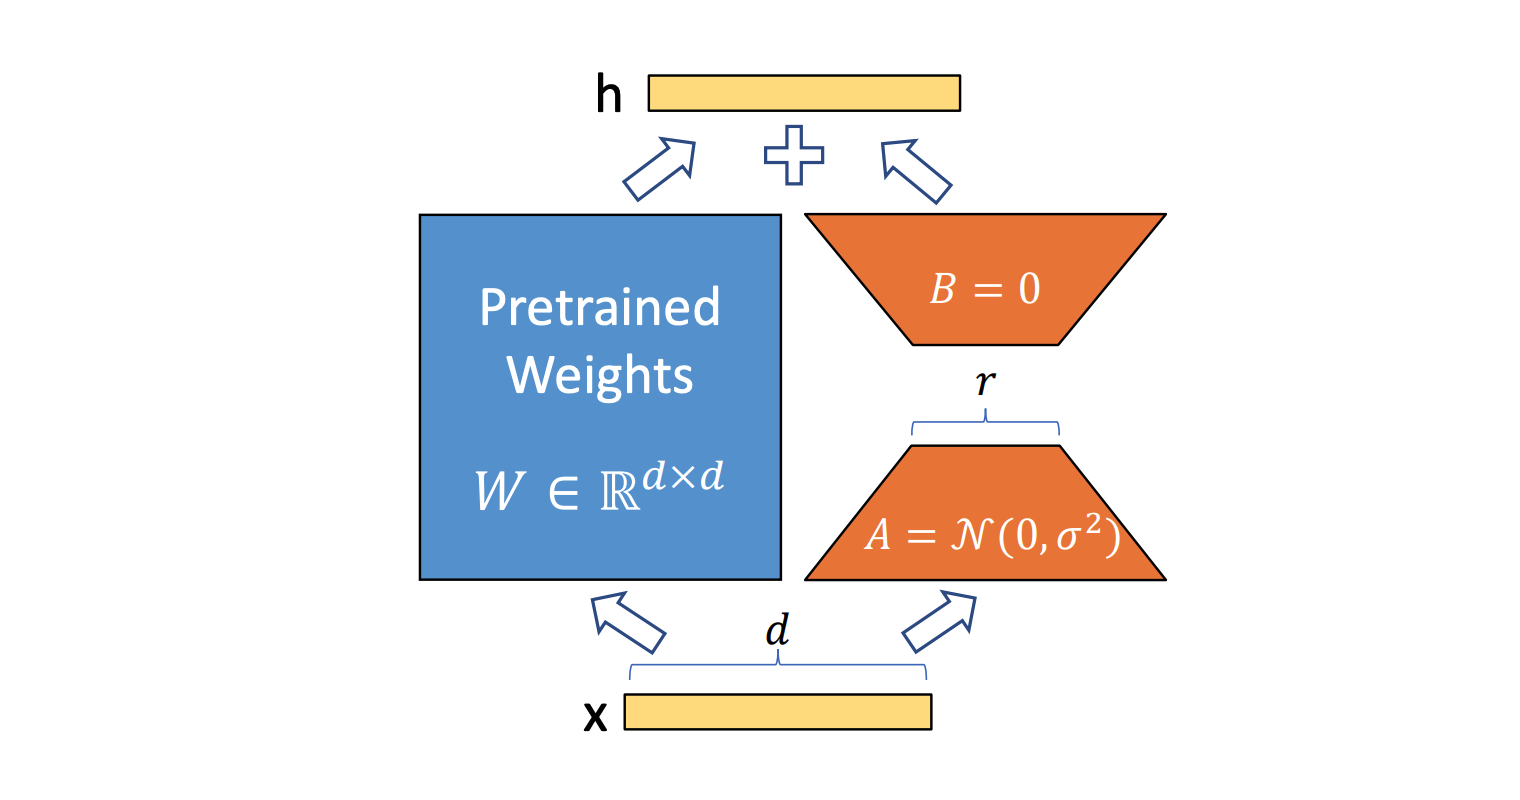
\includegraphics[width=1.0\textwidth]{lora_mechanism.png}
    \captionof{figure}{Cơ chế hoạt động của LoRA. Trọng số gốc $W_0$ được đóng băng. Một nhánh phụ song song được thêm vào, bao gồm hai ma trận thứ hạng thấp $A$ và $B$. Chỉ có $A$ và $B$ được cập nhật trong quá trình huấn luyện.}
    \label{fig:lora_mechanism}
\end{center}

\subsubsection{Lợi ích của LoRA}
\begin{itemize}
    \item \textbf{Hiệu quả về lưu trữ:} Thay vì lưu một bản sao 13 tỷ tham số cho mỗi tác vụ, bạn chỉ cần lưu các ma trận LoRA A và B, có thể chỉ vài megabyte.
    \item \textbf{Chuyển đổi tác vụ nhanh chóng:} Có thể "cắm" và "rút" các adapter LoRA khác nhau vào cùng một mô hình nền tảng để chuyển đổi giữa các tác vụ mà không cần tốn thời gian tải lại toàn bộ mô hình.
    \item \textbf{Không có độ trễ suy luận (Inference Latency):} Sau khi huấn luyện xong, các trọng số LoRA ($BA$) có thể được \textbf{gộp (merged)} vào trọng số gốc ($W = W_0 + BA$). Quá trình suy luận sau đó diễn ra trên một ma trận duy nhất $W$, không có thêm bất kỳ chi phí tính toán nào so với mô hình gốc.
\end{itemize}

\subsection{QLoRA: Lượng tử hóa LoRA (Quantized LoRA)}
\label{ssec:qlora}
QLoRA (Dettmers et al., 2023) \cite{dettmers2023qlora} là một cải tiến đột phá của LoRA, giúp giảm yêu cầu về bộ nhớ GPU xuống mức cực thấp, cho phép tinh chỉnh các mô hình hàng tỷ tham số trên các GPU dành cho người tiêu dùng.

\subsubsection{Ý tưởng cốt lõi}
QLoRA kết hợp LoRA với một kỹ thuật gọi là \textbf{lượng tử hóa (quantization)}.
\begin{itemize}
    \item \textbf{Vấn đề:} Mặc dù LoRA chỉ huấn luyện một số ít tham số, nó vẫn yêu cầu phải \textbf{tải toàn bộ mô hình gốc vào bộ nhớ GPU} để thực hiện quá trình truyền thẳng (forward pass). Với các mô hình lớn, các trọng số này (thường ở định dạng 16-bit) vẫn chiếm một lượng VRAM khổng lồ.
    \item \textbf{Giải pháp của QLoRA:} Tải mô hình nền tảng đã được \textbf{lượng tử hóa xuống định dạng 4-bit}. Tức là, mỗi trọng số chỉ dùng 4 bit để lưu trữ thay vì 16 bit, giảm yêu cầu bộ nhớ đi 4 lần.
    \item \textbf{Thách thức:} Việc huấn luyện trực tiếp trên các trọng số 4-bit là không ổn định.
    \item \textbf{Sự đột phá của QLoRA:} Nó giới thiệu một kiểu dữ liệu 4-bit mới gọi là \textbf{4-bit NormalFloat (NF4)} và kỹ thuật \textbf{Double Quantization} để giảm thiểu mất mát thông tin. Quan trọng nhất, trong quá trình truyền thẳng, các trọng số 4-bit của mô hình nền tảng được \textbf{giải lượng tử hóa (de-quantized) về định dạng 16-bit "ngay khi cần"} cho việc tính toán, sau đó bị loại bỏ khỏi bộ nhớ. Gradient vẫn được lan truyền ngược qua các adapter LoRA ở định dạng 16-bit.
\end{itemize}

Nhờ QLoRA, việc tinh chỉnh một mô hình 65 tỷ tham số có thể được thực hiện trên một GPU duy nhất với 48GB VRAM, một điều không tưởng trước đây.

\subsection{Adapter-tuning}
\label{ssec:adapter_tuning}
Đây là một trong những họ phương pháp PEFT \cite{houlsby2019parameter} đầu tiên, có trước cả LoRA.
\begin{itemize}
    \item \textbf{Kiến trúc:} Thay vì thêm các nhánh song song, Adapter-tuning chèn các module nhỏ, gọi là \textbf{các lớp adapter (adapter layers)}, vào \textbf{bên trong} mỗi khối Transformer, thường là sau lớp Multi-Head Attention và lớp FFN.
    \item \textbf{Cơ chế:} Các lớp adapter này thường có kiến trúc "cổ chai" (bottleneck): một lớp tuyến tính giảm chiều, một hàm kích hoạt phi tuyến, và một lớp tuyến tính tăng chiều trở lại.
    \item \textbf{Huấn luyện:} Tương tự, toàn bộ mô hình gốc được đóng băng và chỉ có các tham số của các lớp adapter này được huấn luyện.
    \item \textbf{So với LoRA:} Adapter có nhược điểm là chúng thêm vào độ trễ suy luận vì đầu ra phải đi qua các lớp bổ sung một cách tuần tự. LoRA khắc phục được điều này nhờ khả năng gộp trọng số.
\end{itemize}

\subsection{Prompt-based Tuning: Điều chỉnh trên Lớp Đầu vào}
\label{ssec:prompt_tuning}
Các phương pháp trên can thiệp vào trọng số của mô hình. Một hướng tiếp cận khác, cấp tiến hơn, là: \textbf{giữ nguyên hoàn toàn mô hình và chỉ điều chỉnh đầu vào}.

\subsubsection{Prompt-Tuning}
\begin{itemize}
    \item \textbf{Ý tưởng:} Thay vì tinh chỉnh các trọng số khổng lồ, hãy học cách tìm ra "prompt" tốt nhất cho mô hình. Nhưng thay vì tìm kiếm các từ trong ngôn ngữ tự nhiên (hard prompt), Prompt-Tuning \cite{lester2021power} học một chuỗi các \textbf{vector embedding "mềm" (soft prompts)} liên tục.
    \item \textbf{Cơ chế:} Một số lượng nhỏ ($k$) các vector prompt có thể huấn luyện được sẽ được \textbf{chèn vào phía trước} chuỗi embedding đầu vào. Toàn bộ mô hình gốc được đóng băng. Trong quá trình huấn luyện, chỉ có các vector prompt này được cập nhật thông qua lan truyền ngược.
    \item \textbf{Lợi ích:} Cực kỳ hiệu quả về tham số (chỉ cần học vài nghìn tham số) và dễ dàng lưu trữ, chia sẻ các "prompt" đã được học cho các tác vụ khác nhau.
\end{itemize}

\subsubsection{Prefix-Tuning}
\begin{itemize}
    \item \textbf{Ý tưởng:} Tương tự Prompt-Tuning, nhưng thay vì chỉ chèn các vector vào lớp embedding đầu vào, Prefix-Tuning \cite{li2021prefix} chèn các tiền tố (prefixes) có thể huấn luyện được vào \textbf{mỗi lớp Transformer} của mô hình.
    \item \textbf{Cơ chế:} Các tiền tố này hoạt động như một "ngữ cảnh ảo" dành riêng cho tác vụ, giúp điều khiển hành vi của mỗi lớp một cách trực tiếp hơn.
    \item \textbf{Hiệu năng:} Thường cho kết quả tốt hơn Prompt-Tuning nhưng có nhiều tham số hơn để huấn luyện.
\end{itemize}

Các kỹ thuật PEFT đã thay đổi hoàn toàn cách chúng ta làm việc với LLMs, giúp việc tùy chỉnh các mô hình khổng lồ trở nên khả thi, tiết kiệm và linh hoạt hơn bao giờ hết.